\documentclass[12pt]{article}

\usepackage{sbc-template}

\usepackage{graphicx,url}

\usepackage{mathtools}

\usepackage[brazil]{babel}   
\usepackage[utf8]{inputenc}  

\usepackage[autostyle]{csquotes}  
     
\sloppy

\title{Sistema de Recomendação Baseado em Confiança para Promover a Colaboração em Redes de Pesquisa Científica}

\author{João Pedro R. D. Saldanha\inst{1}, Fernando Prass\inst{1}}


\address{Ciência da Computação -- Universidade Franciscana (UFN)\\
  Rua dos Andradas, 1614  -- 97010-032  -- Santa Maria -- RS -- Brasil
\email{\{joao.pedro,fernando.prass\}@ufn.edu.br}
}

\begin{document} 

\maketitle

\begin{abstract}
  This meta-paper describes the style to be used in articles and short papers
  for SBC conferences. For papers in English, you should add just an abstract
  while for the papers in Portuguese, we also ask for an abstract in
  Portuguese (``resumo''). In both cases, abstracts should not have more than
  10 lines and must be in the first page of the paper.
\end{abstract}
     
\begin{resumo} 
  Este meta-artigo descreve o estilo a ser usado na confecção de artigos e
  resumos de artigos para publicação nos anais das conferências organizadas
  pela SBC. É solicitada a escrita de resumo e abstract apenas para os artigos
  escritos em português. Artigos em inglês deverão apresentar apenas abstract.
  Nos dois casos, o autor deve tomar cuidado para que o resumo (e o abstract)
  não ultrapassem 10 linhas cada, sendo que ambos devem estar na primeira
  página do artigo.
\end{resumo}


\section{Introdução}

No método científico, pesquisadores devem realizar um trabalho criativo sistemático para incrementar 
o conhecimento na área da pesquisa. Parte importante do processo é a busca, dentro do universo dos 
trabalhos científicos, por embasamento teórico ao tema do trabalho proposto. Além disto, também é 
relevante conhecer e colaborar com pesquisadores desenvolvendo trabalhos relacionados dentro da 
área de pesquisa.  Portanto, é preciso reunir todas as informações pertinentes, pesquisas e resultados 
anteriores bem como linhas de pesquisa em progresso para não reinventar a roda ou seguir caminhos já 
trilhados e assim realizar trabalho relevante e produtivo.

A plataforma Lattes é um sistema que integra bases de dados de currículos, em específico de pesquisadores. 
Ela oferece aos usuários a possibilidade de criar um currículo de maneira gratuita, que é disponibilizado 
abertamente aos visitantes do site. Segundo \cite{CNPq2019lattes}, o Currículo Lattes 
\textit{"se tornou um padrão nacional no registro da vida pregressa e atual dos estudantes e 
pesquisadores do país, e é hoje adotado pela maioria das instituições de fomento, universidades e 
institutos de pesquisa do País"}.
    
O universo da pesquisa científica está em constante expansão, tanto no que diz respeito ao conhecimento 
produzido quanto ao volume de trabalhos e publicações. Estimativas apontavam um valor em torno de 2.5 
milhões de artigos científicos publicados por ano, em 2015, com um aumento de 5\% ao ano no número de 
cientistas fazendo publicações \cite{ware2015stm}. Pesquisadores não têm o tempo necessário para analisar 
todos os estudos relacionados à seus próprios trabalhos, mesmo com plataformas como o Lattes, onde estão 
tais trabalhos estão compilados. Trata-se do problema da sobrecarga de informação, que tem crescido na 
medida em que sistemas digitais vem ganhando cada vez usuários e conteúdo. Outro problema decorrente do 
crescimento do número de pesquisadores e trabalhos é que muitas vezes os pesquisadores não conhecem outros 
pesquisadores da área e acabam por perder a oportunidade de colaborações ou troca de idéias.

Logo, se faz necessário a filtragem da informação que chega ao pesquisador para maximizar sua eficiência e 
evitar tempo perdido. A automatização de tal tarefa de filtragem pode ser feita através de sistemas de recomendação, 
utilizando técnicas de mineração de dados e inteligência artificial para oferecer o conteúdo mais relevante 
disponível, aumentando a eficiência do acadêmico. 

A partir do problema da sobrecarga de informações, nos anos 90 iniciou-se a pesquisa na área de filtragem de conteúdo. 
O ponto de partida foi a observação que as pessoas usam, no dia-a-dia, dicas de outros para tomar decisões, sendo que 
as dicas daqueles tidos como especialistas no assunto tem um peso diferenciado. Os primeiros sistemas de recomendação 
eram algoritmos capazes de analizar tendências dentro de uma certa comunidade e então fazer sugestões aos seus membros. 
Este método é conhecido como filtragem colaborativa e foi aprimorado desde então, sendo até hoje bastante popular. Além 
deste, também é bastante difundido o método baseado em conteúdo, no qual novos itens são recomendados baseado no 
conteúdo consumido pelo usuário no passado \cite{ricci2011introduction}.

\subsection{Objetivos}

Neste trabalho é proposta a elaboração de um sistema de recomendações de pesquisadores e trabalhos científicos baseado 
em confiança a partir de dados da plataforma lattes. A ideia é analisar o sentimento da comunidade em relação a cada
pesquisador e sugerir conteúdo relevante aos pesquisadores baseado em seus perfis, ponderando o conteúdo com base na 
confiança estimada da comunidade. Para tal, é preciso:

\begin{itemize}
  \item Estudar funções e aplicações de sistemas de recomendação
  \item Modelar a rede de confiança da comunidade científica
  \item Estabelecer métricas eficientes de confiança para os dados disponíveis
  \item Estimar a confiança entre os pesquisadores 
  \item Pré-selecionar recomendações
  \item Filtrar a pré-seleção com a confiança computada
  \item Avaliar o modelo
\end{itemize}

\subsection{Proposta}

Para solucionar o problema explanado, a proposta é descrever uma rede de colaborações baseada nas publicações em conjunto, 
discutida na seção \ref{sect:computing-trust} utilizando técnicas encontradas na literatura para computar a propagação de 
confiança na rede. Para isso são discutidas três métricas na seção \ref{sect:computing-trust}. A partir daí, é discutida a 
pré seleção dos itens com o método baseado em conteúdo(seção \ref{sect:pre-selection}), proposta uma arquitetura para o sistema 
de recomendações (seção \ref{sect:arch}) e uma metodologia para sua validação (seção \ref{sect:validation}).

\section{Revisão Bibliográfica}

Nesta seção, será feita a apresentação dos principais itens que compõem o  embasamento teórico usado como ponto de 
partida no trabalho e usado para justificar as decisões tomadas.

\subsection{Sistemas de Recomendação (SR)}

Frequentemente usuários de plataformas digitais se deparam com situações nas quais é necessário escolher entre 
vários itens ofertados: Produtos, conteúdo ou pessoas. A dificuldade de filtrar o conteúdo encontrado em determinada 
plataforma tende a aumentar na medida em que o número de itens ofertados cresce, visto que é necessário fazer uma 
análise individual de tais itens e então compará-los para fazer uma escolha. Para ajudar na tarefa, é comum encontrar 
sistemas que automatizam o processo de escolha, filtrando o conteúdo com base no perfil do usuário para apresentar 
seu interesse. Tais sistemas são especificamente úteis quando um usuário encontra dificuldades para analisar os itens 
ofertados e fazer escolhas. Os itens recomendados pelos SR podem ser os mais variados, sendo que no geral a recomendação 
é uma tarefa especializada, ou seja, apenas um tipo de item é recomendado, e a recomendação é relevante para um perfil 
específico de usuário. Logo, as características do SR, como metodologia usada para sua construção, interface de usuário 
e critério para ordenar os resultados devem ser adaptados às especificidades da tarefa em questão. 

A forma mais simples do resultado de um SR é uma lista de itens ordenada de acordo com a preferência do usuário. A satisfação 
com as recomendações pode ser coletada explicitamente, como por exemplo através de avaliações, ou implicitamente através de 
inferências baseadas no comportamento do usuário perante aos itens oferecidos. Para oferecer recomendações, é preciso analisar 
uma base de conhecimento, que pode ter diversas informações, realizar um trabalho de classificação dos itens ofertados e 
então coletar algum tipo de feedback perante o resultado que deve ser usado para aprimorar o sistema \cite{ricci2011introduction}.

\subsubsection{Técnicas de Recomendação}

O resultado obtido por um SR é dependente da realização de uma \textbf{predição}. A predição é fundamental para a qualidade 
das recomendações: Itens são apresentados ao usuário porque  o sistema antecipa que sejam relevantes para ele 
\cite{ricci2011introduction}. Geralmente na elaboração de sistemas de recomendação lida-se com \textbf{usuários}, denotados por 
$ u_1, ... u_n \in U $, \textbf{itens}, denotados por $ i_1, ... i_n \in I$  e \textbf{relações}, que associam usuários e 
itens de diversas maneiras \cite{ekstrand2019recommender}. As associações podem ser representadas por ontologias 
\cite{primo2006tecnicas} ou no caso de relações entre usuários e itens através de uma matriz de associação $ |U| \times |I| $. 
Assume-se a existência no mundo real de uma \textbf{função} $ f (u, i) $ que retorne um número real representado a utilidade do 
item $i$ ao usuário $u$. Em técnicas de filtragem colaborativa, este numero é visto como a avaliação do usuário. A tarefa do SR 
neste contexto é computar uma função $\hat{f}(u, i)$ que se assemelhe ao máximo à $f$. 
Assim, é possível realizar a predição de relevância de um grupo de itens para determinado usuário $\hat{f}(u_n, I)$ e recomendar 
os itens melhores classificados pelo SR, efetivamente filtrando o conteúdo e oferecendo ao usuário uma seleção personalizada de 
itens \cite{ricci2011introduction}.

\subsubsection{Filtragem Colaborativa}

Técnicas de filtragem colaborativa analisam o \textbf{perfil} do usuário e sua \textbf{avaliação} dos itens previamente 
acessados para chegar em recomendações. Procura-se analisar o perfil do \textbf{usuário alvo} para então achar um \textit{cluster} 
de usuários com perfis similares (\textbf{vizinhos}). A idéia é que os itens bem avaliados pelos vizinhos serão também 
avaliados positivamente pelo usuário alvo, já que os perfis são semelhantes. Um problema encontrado na técnica é o problema 
da primeira avaliação: Quando há um item novo, sem nenhuma avaliação, como saber se determinado usuário irá avaliar 
positivamente o item? Nenhum de seus vizinhos fez avaliações \cite{ricci2011introduction}.

SRs baseados em filtragem colaborativa são os mais populares na área e vêm sido pesquisados há mais tempo. \cite{ricci2011introduction} 
É comum utilizar métodos baseados em vizinhança, nos quais um algoritmo de clusterização é usado para determinar grupos 
de usuários ou ítens, tal como o algoritmo \textbf{KNN} (\textit{K-Nearest Neighbours}) \cite{da2018desenvolvimento}.

\subsubsection{Método Baseado em Conteúdo}

O método baseado em conteúdo parte da idéia de que usuários têm interesse em itens semelhantes àqueles que lhe foram uteis 
no passado \cite{ricci2011introduction}. No caso, é importante determinar a \textbf{semelhança entre itens} para então recomendar 
para determinado usuário itens semelhantes aos que foram \textbf{previamente bem avaliados} por ele. Nesse método, 
é preciso estabelecer estratégias para descrever itens bem como para montar o perfil dos usuários, descrevendo os tipos 
de itens que ele tem interesse em. Então, deve ser feito o \textbf{comparativo} dos itens com o perfil do usuário para 
predizer seu interesse em tais itens. Geralmente procura-se dividir o universo dos itens, $I$, em categorias: Relevantes ou 
irrelevantes ao usuário, por exemplo. Para  construir a classificação dos itens, é possível usar uma série de algoritmos que 
realizam trabalho de \textbf{classificação estatística}, como por exemplo \textbf{árvores de decisão} \cite{pazzani2007content}. 

\subsubsection{Método Baseado em Confiança}

Estudos indicam que os usuários têm a tendência de \textbf{valorizar mais as recomendações de amigos} do que aquelas feitas 
por outros usuários com perfil semelhante, porém desconhecidos e a qualidade das recomendações de amigos superam inclusive 
as feitas por sistemas de recomendação \cite{sinha2001comparing}. A partir deste conceito, com a grande aderência de usuários 
à \textbf{redes sociais} um novo método para a construção de sistemas de recomendação está sendo estudado. Trata-se do método 
baseado em confiança, ou sistema de recomendação social (\textit{social recommender system}) \cite{ricci2011introduction}.

A construção de SRs sociais depende do estabelecimento de uma \textbf{rede de confiança}, ou seja, uma rede social que descreve 
o nível de confiança entre seus membros. Assim, o usuário recebe recomendações de itens avaliados positivamente por usuários 
em sua rede de confiança. Estes SRs precisam usar o conceito de \textbf{agregação e dissipação de confiança}, ou seja, 
dados um grupo de usuários $u_1  \dots u_n$, calcular o nível de confiança entre $u_1$ e $u_n$ considerando usuários intermediários
$u_2 \dots u_{n-1}$ que possuem alguma relação de confiança, direta ou indireta, com $u_1$ e $u_n$ (\textbf{dissipação}) ou 
combinar uma série de estimativas de confiança em um valor final (\textbf{agregação}) \cite{victor2011trust}.

Um ponto fraco de tais sistemas é que a recomendação é geralmente mais previsível e pode facilmente ser inundada por itens que o 
usuário já conhece, enquanto técnicas mais usuais de recomendação podem apresentar resultados mais inesperados, mas relevantes ao 
usuário \cite{sinha2001comparing}.

\subsubsection{Métodos Híbridos}

\subsection{Trabalhos Correlatos}

Os trabalhos correlatos foram escolhidos utilizando como critério a contemporaneidade e semelhança com o presente trabalho, 
de forma a trazer um embasamento atualizado das metodologias usadas para a resolução de problemas semelhantes.

\subsubsection{Desenvolvimento de um Sistema de Recomendação para Bibliotecas Digitais}

Este trabalho também aborda o problema da sobrecarga de informações dos pesquisadores baseando-se no perfil do currículo lattes. 
O trabalho busca recomendações de produções científicas utilizando o motor de buscas google acadêmico e traz uma combinação 
das técnicas de filtragem colaborativa e baseado em conhecimento. A metodologia para gerar recomendações utilizada neste 
trabalho será usada no presente trabalho como referência para a elaboração do SR, levando em consideração os pontos fracos 
e fortes da abordagem descrita no trabalho. Em particular, será considerada a maneira com que o trabalho propôs solucionar 
o problema  da avaliação inicial de um SR de filtragem colaborativa através do método baseado em conteúdo \cite{da2018desenvolvimento}.

\subsubsection{Técnicas de Recomendação para usuários de Bibliotecas
Digitais}

Trabalho que apresenta algumas das mais populares técnicas de recomendação, bem como a justificativa e contexto para a 
correta implementação dos mesmos. O trabalho descreve diversas abordagens para a elaboração de um SR de obras literárias 
em bibliotecas digitais, usando as técnicas de filtragem colaborativa e baseado em conteúdo bem como uma abordagem híbrida. 
O contexto do sistema de recomendação descrito no trabalho se assemelha ao do presente trabalho por ter como alvo uma 
biblioteca digital, sendo que as obras literárias da biblioteca podem ser comparadas aos artigos encontrados na plataforma 
lattes. O comparativo das metodologias usadas serve como referência para a elaboração do SR descrito no presente trabalho. 
As relações entre usuário e items (no caso, obras literárias) é descrita através de uma ontologia na qual conceitos são 
definidos pelos termos que os definem e organizados em uma hierarquia. A ontologia serve para descrever as relações entre 
item e usuário e serve como referência para a modelagem das relações do SR desenvolvido neste trabalho. O trabalho também 
apresenta um experimento para ilustrar a importância da opinião de especialistas \cite{primo2006tecnicas}.

\subsubsection{Trust-aware Collaborative Filtering for Recommender Systems}

\section{Materiais \& Métodos}

Para chegar nas recomendações, é proposto um trabalho em dois momentos: estimar a confiança entre pesquisadores e então
selecionar potenciais colaboradores baseando-se no perfil dos pesquisadores. A seleção será filtrada e ordenada de acordo com o 
nível de confiança estimado dos pesquisadores. O primeiro passo é modelar uma rede de confiança da comunidade científica, descrita 
por autores e publicações. Pode então ser feita uma seleção dos pesquisadores cadastrados com base no perfil do usuário alvo e 
ordenar a seleção de acordo com o nível de confiança de cada pesquisador. A confiança pode ser local ou global, sendo que local diz 
respeito à confiança estimada de um pesquisador específico em seus colegas e a global corresponde à a confiança da comunidade em 
cada pesquisador. Em termos de ferramentas para implementação, foi escolhida a linguagem Python, que possui riqueza de ferramentas 
e recursos para trabalhos relacionados a manipulação de dados e computação numérica.% \cite{python book} 

\subsection{Os Dados da Plataforma Lattes}

Os dados usados no trabalho são provenientes de um banco de dados relacional extraído do currículo lattes dos pesquisadores com o 
uso de um \textit{parser}. O parser descrito em \cite{prass2019parser} oferece uma interface para a extração automatizada de dados 
da plataforma lattes. A partir dos arquivos \textit{XML} exportados da plataforma, o \textit{parser} faz uma análise a partir da 
qual são montadas relações entre os itens presentes no banco e os novos itens, relacionando autores às suas publicações cadastradas, 
ou seja, inserindo uma linha em uma tabela associativa entre autor e publicação, conforme a Figura \ref{fig:database}. A partir do banco descrito, é 
possível construir uma base de conhecimento focada especificamente no objetivo do presente trabalho, que é descrita a seguir.

\begin{center}
  \begin{figure}[ht]
    \centering
    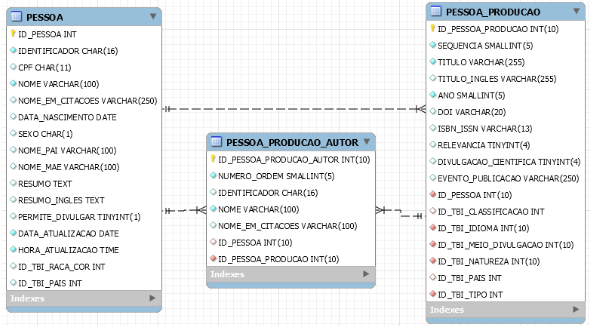
\includegraphics[width=.8\textwidth]{database.png}
    \caption{Tabelas Pessoa, Produção e associativa \cite{prass2019parser}}
    \label{fig:database}
  \end{figure}
 \end{center}

\subsubsection{Publicações}

Uma publicação científica, normalmente, é uma produção de algum \textbf{tipo} (artigo, livro, trabalho) que passou por um processo de 
revisão por pares e foi aceito como sendo uma contribuição válida, de autoria de um ou mais pesquisadores. A maioria das 
publicações da base de conhecimento possuem alguma \textbf{palavra-chave}, informada pelos autores, que servem como uma pista 
dos assuntos abordados. As publicações são feitas originalmente em um \textbf{idioma} e \textbf{país} específicos e 
obrigatoriamente possuem um \textbf{título} no idioma original bem como uma possível tradução para o inglês. O \textbf{ano} da 
publicação é considerado relevante devido à característica progressiva do conhecimento científico, onde observa-se constante 
introdução de novos dados e fatos. Em alguns casos é possível inferir a \textbf{abrangência} da publicação, por exemplo pode 
ser regional, nacional ou internacional. Algumas tuplas podem também conter a \textbf{natureza}, que deve ser vista como o 
nível de cobertura do assunto discutido alcançado pelo trabalho: Completo, resumo e assim por diante. A ordem dos nomes dos 
autores geralmente é indicativo da importância do autor para a publicação: O \textbf{autor principal} geralmente é o primeiro 
nome, e o \textbf{orientador} do trabalho o último. Entre eles, os colaboradores \textbf{intermediários}.  

\subsubsection{Pesquisadores}

Os autores são o centro dos dados da base de conhecimento e são também responsáveis por cadastrar todas as informações lá 
encontradas. O perfil do pesquisador é composto por sua \textbf{formação}, \textbf{atuação profissional}, e 
\textbf{publicações} das quais fez parte. A formação é representada por um título, que diz respeito ao nível de ensino, por 
exemplo doutorado ou mestrado. 


\subsection{Computando confiança} \label{sect:computing-trust}

Pode-se pensar na rede de confiança como sendo um grafo no qual os nodos são pesquisadores e as arestas publicações em conjunto.
Considerando que uma colaboração em publicações é um voto de confiança entre os pesquisadores envolvidos, a matriz de adjacência 
pode ser usada para computar a propagação de confiança através da rede. A confiança estimada de determinado pesquisador deve levar 
em consideração o nível de confiança estimado dos pesquisadores que colaboraram com ele.

O algoritmo PageRank \cite{page1999pagerank} foi inspirado em parte por estudos realizados em redes de citações acadêmicas, nas 
quais a relevância de um artigo era descrita por contagem de citações, por exemplo. Trata-se de um método para computar um \textit{ran\-king} 
global de citações, pensado para computar a importância das paginas web. O \textit{ranking} $R$ de uma página é definido como a soma dos 
\textit{rankings} das páginas que oferecem links para ela, ponderada pelo total de \textit{links} encontrados nas páginas.

É definido para cada página $u$ um conjunto $F_u$ de páginas as quais $u$ referencia e um conjunto $B_u$ de páginas que fazem 
referência à $u$. Sendo $\hat{A}$ a matriz de adjacência da web, tal que 

\[ \hat{A}_{i,j} =
  \begin{cases}
    1       & \quad \text{se } \text{ há links de i para j}\\
    0       & \quad \text{se } \text{ não há links de i para j}
  \end{cases}
\]

A matriz $A$ deve ser obtida dividindo todas as linhas de $\hat{A}$ por $|F_u|$ (o grau do nodo $u$). Assim, PageRank pode ser definido 
como $R = c(AR + E)$, sendo $c$ um fator de normalização.

Quando ocorrem ciclos no fluxo de referência, nos quais duas páginas se referenciam mutuamente e não fazem referência a nenhuma 
outra página, pode ocorrer o chamado \textit{rank sink} quando há referencias exteriores injetando \textit{ranking} no ciclo, 
assim as páginas do ciclo acumulam ranking, porém não há distribuição. Para solucionar, foi introduzido o vetor $E$, que no modelo 
de PageRank é o conceito de um \textit{random surfer}, ou seja, uma probabilidade de um usuário da internet aleatoriamente mudar a 
página, sem seguir nenhum de seus \textit{links}. \cite{page1999pagerank}

A aplicação de PageRank à um grafo não-direcionado gera um vetor $R$ estatisticamente similar à distribuição de grau dos nodos da 
rede \cite{perra2008spectral}. Isto é, aplicando diretamente o algoritmo ao problema proposto, no final das contas a confiança 
seria proporcional ao número de publicações do autor (\textbf{centralidade} do nodo). Enquanto esta métrica é relevante, perde-se 
a idéia inicial: Não é considerada a confiança dos colaboradores, somente o valor total de colaborações. 

Além disso, alguns conceitos importantes não são levados em consideração: A relevância e o número de colaborações entre os 
pesquisadores. No caso da \textbf{relevância}, a importância da publicação é uma dica para o nível de confiança mútua entre os 
pesquisadores: colaborações em publicações importantes requerem maior confiança. O total de \textbf{colaborações em conjunto} 
entre um par de pesquisadores, por sua vez, indica uma relação mais duradoura, com mais confiança mútua. É importante distinguir 
total bruto de publicações de determinado pesquisador e o número de colaborações entre dois pesquisadores, pois há mais confiança 
quando observa-se frequentes colaborações.  Uma vez estabelecida uma heurística para a importância de determinada colaboração, 
pode-se somar as importâncias para avaliar a força dos laços de confiança.

\subsubsection{Relevância}

Nem todas as publicações são feitas iguais. É possível considerar as características descritas na representação de publicação 
usada na base de conhecimento para construir uma heurśtica sobre a relevância da publicação. Pesos podem ser atribuidos para os 
atributos contidos na tabela publicação. Aqui, a heurística considerada é a natureza da publicação, com pesos atribuidos conforme 
a tabela \ref{tab:relavancy}.

\begin{center}
  \begin{table}[ht]
    \centering
    \caption{Heurśtica de Relevância}
    \label{tab:relavancy}
    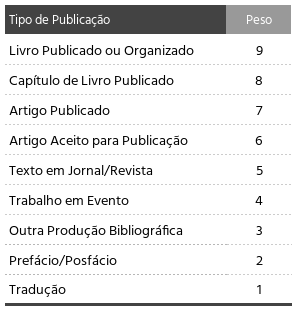
\includegraphics[width=.4\textwidth]{heuristics.png}
    \end{table}
\end{center}

\subsubsection{Centralidade}

Considerando as heurísticas definidas, é possível alcançar um fluxo de confiança mais interessante na rede modelada. O conceito 
de agregação e dissipação de confiança pode seguir a idéia do algoritmo \textit{PageRank} aplicando-se um algoritmo para o 
cálculo da centralidade dos nodos. Assim, a relevância das publicações e a quantidade de colaborações podem ser levadas em 
consideração na distribuição de confiança.

Várias métricas foram propostas na literatura para o cálculo da centralidade, em especial a proposta em \cite{opsahl2010node} 
se encaixa particularmente bem no problema proposto por incorporar simultaneamente o grau (número de conexões) e a força 
(os pesos de cada conexão) dos nodos. Aqui, o peso pode ser a soma das relevâncias das obras publicadas em conjunto entre os 
pesquisadores. A fórmula proposta faz isso definindo um parâmetro $\alpha$ para ajustar a importância de grau e força:

\begin{center} 
  $ C_D ^{w \alpha} (i) = k_i \times \left( \frac {s_i} {k_i} \right) ^{\alpha} = k_i ^{1 - \alpha} \times s _i ^{\alpha} $
\end{center}

Ao incorporar o número e a relevância das publicações como um peso para as arestas da rede, é reintroduzido o conceito de 
considerar a confiança da comunidade nos colaboradores que depositaram confiança em determinado autor através de publicações 
em  conjunto para o cálculo da confiança estimada de tal autor. Assim, é possível chegar em um fluxo de confiança apurado 
levando em conta informações sobre obras e autores que são relevantes para considerar a confiança compartilhada entre 
os membros da rede.

\subsubsection{Distância}

\subsubsection{Confiança subjetiva}

Uma alternativa aos métodos descritos acima é transformar a rede de confiança em um grafo direcionado. Pode-se chegar nesse objetivo 
gerando uma rede de confiança para cada pesquisador ao qual se deseja fazer recomendações. Com essa técnica, a aplicação direta 
de PageRank à rede de confiança pode gerar um resultado significativo.

Sejam $F$ e $B$ conjuntos de colaboradores, conforme definido em PageRank, $G_{u}^{0}$ o usuário alvo $u$ e $B_{u}^{0}$ também o 
usuário $u$. O conjunto dos colaboradores diretos de $u$, aqueles com os quais $u$ possui publicações em conjunto, são definidos 
como $G_{u}^{1}$ e os colaboradores dos colaboradores de $u$ são o conjunto $G_{u}^{2}$. Pode-se generalizar os colaboradores 
de grau $n (n \geq 1)$ como o seguinte:

\begin{center}
  $ G_{u}^{n} = v | v \in F_{G_{u}^{n}}, v \notin B_{G_{u}^{n-1, n-2 \dots 0}} $
\end{center}

Assim, $F_{G_{u}^{n}}$ e $B_{G_{u}^{n-1, n-2 \dots 0}}$ ambos  representam um grupo de pesquisadores que publicaram obras em conjunto 
com os pesquisadores do conjunto $G_{u}^{n}$, considerado um voto de  confiança. A diferença é que os pesquisadores do conjunto 
$B_{G_u^{n-1, n-2 \dots 0}}$ já apareceram na rede de confiança de $u$.

Pode-se a partir dessa definição escrever uma função capaz de estabelecer recursivamente a rede de confiança relativa de 
determinado pesquisador, iterando sobre os pesquisadores envolvidos  em colaborações diretas até que $ G^{n}_{u} $ seja um 
conjunto vazio. Vale notar que embora essa técnica seja consideravelmente mais intensiva em termos de computação quando o objetivo 
é calcular a confiança relativa para todos os pesquisadores do sistema, o algoritmo PageRank converge rapidamente mesmo para 
grandes quantidades de páginas \cite{page1999pagerank}.

Nesse caso, é computada a confiança local, ou seja, a confiança estimada de cada pesquisador em relação aos outros pesquisadores, 
e não a confiança estimada da comunidade como um todo em cada pesquisador.

\subsection{Pré-seleção de Recomendações} \label{sect:pre-selection}

Com as métricas de confiança propostas acima, é possível estabelecer níveis de confiança da comunidade, uma rede subjetiva do 
pesquisador alvo ou distâncias ponderadas por confiança e usar as predições para oferecer sugestões de colaboradores para cada 
membro da rede em diferentes contextos. Todavia confiança apenas pode não ser suficiente para recomendações de qualidade. 
Considerar também a linha de pesquisa do pesquisador no momento e os perfis dos potenciais colaboradores pode aumentar a qualidade 
das recomendações: Mesmo que a confiança em um pesquisador seja alta, a sugestão de colaboração pode não fazer sentido caso as 
linhas de pesquisa não se encaixem.

Para augmentar as recomendações, é proposta uma simples pré-seleção dos itens utilizando um método baseado em conteúdo. A 
técnica proposta consiste no cálculo de correspondência de palavras chave em um modelo de espaço vetorial (MEV), visto que 
esta é a mais comum em sistemas de recomendação baseados em conteúdo \cite{ricci2011introduction}. No MEV proposto, a idéia é estabelecer um 
perfil geral dos pesquisadores através de palavras chaves ponderadas por relevância, extraídas dos títulos e palavras chaves 
das publicações do qual o autor fez parte. O perfil do pesquisador é representado por um vetor em um espaço \textit{n-dimensional}: 
$d_j = {w_{1,j}, w_{2,j}, \dots ,d_{n,j}}$, no qual $w_{i,j}$ representa o quanto o termo $i$ é relevante dentro do trabalho do 
pesquisador $j$. Pode-se pensar em uma matriz na qual as linhas são pesquisadores, conforme descrito e as colunas representam os 
termos-chave extraídos do universo das publicações (\textit{corpus}), removendo palavras vazias - “ou”, “de”, “para” \dots - 
tanto em português quanto em inglês.

Tal matriz é construída através da técnica de vetorização \textit{TF-IDF}, na qual considera-se termos importantes aqueles que 
aparecem com frequência relacionados á um item específico e com menor frequência nos outros itens do \textit{corpus} 
\cite{pazzani2007content}. A partir disso é preciso computar a semelhança entre termos. Para tal, a proposta é o uso da 
similaridade de cossenos por ser a técnica mais comumente aplicada \cite{ricci2011introduction}. Para a pré-seleção dos itens, então, a 
proposta é basear-se em uma \textit{query} que representa o trabalho sendo desenvolvido pelo pesquisador no presente. A partir 
desta, pode-se calcular as similaridades dos perfis dos autores cadastrados com a \textit{query}, construindo assim a pré-seleção.

\subsection{Arquitetura} \label{sect:arch}


\subsection{Validação} \label{sect:validation}

%\section{Figures and Captions}\label{sec:figs}


%Figure and table captions should be centered if less than one line
%(Figure~\ref{fig:exampleFig1}), otherwise justified and indented by %0.8cm on
%both margins, as shown in Figure~\ref{fig:exampleFig2}. The caption font must
%be Helvetica, 10 point, boldface, with 6 points of space before and after each
%caption.

%\begin{figure}[ht]
%\centering
%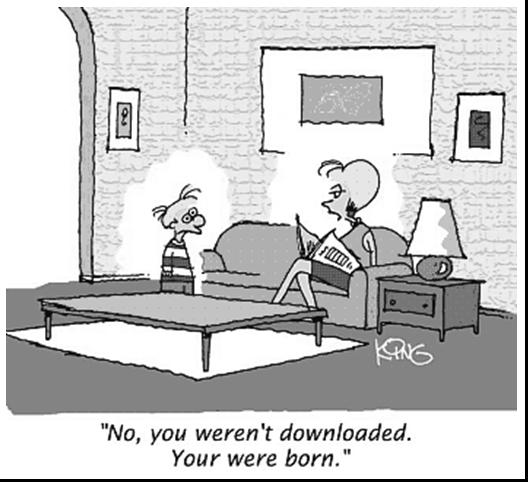
\includegraphics[width=.5\textwidth]{fig1.jpg}
%\caption{A typical figure}
%\label{fig:exampleFig1}
%\end{figure}

%\begin{figure}[ht]
%\centering
%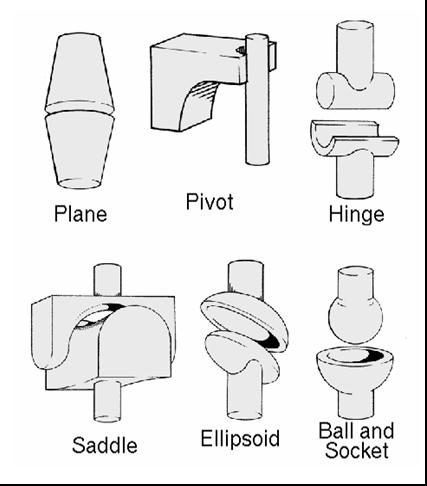
\includegraphics[width=.3\textwidth]{fig2.jpg}
%caption{This figure is an example of a figure caption taking more than one
%  line and justified considering margins mentioned in Section~\ref{sec:figs}.}
%\label{fig:exampleFig2}
%\end{figure}

%In tables, try to avoid the use of colored or shaded backgrounds, and avoid
%thick, doubled, or unnecessary framing lines. When reporting empirical data,
%do not use more decimal digits than warranted by their precision and
%reproducibility. Table caption must be placed before the table (see Table 1)
%and the font used must also be Helvetica, 10 point, boldface, with 6 points of
%space before and after each caption.

%\begin{table}[ht]
%\centering
%\caption{Variables to be considered on the evaluation of interaction
%  techniques}
%label{tab:exTable1}
%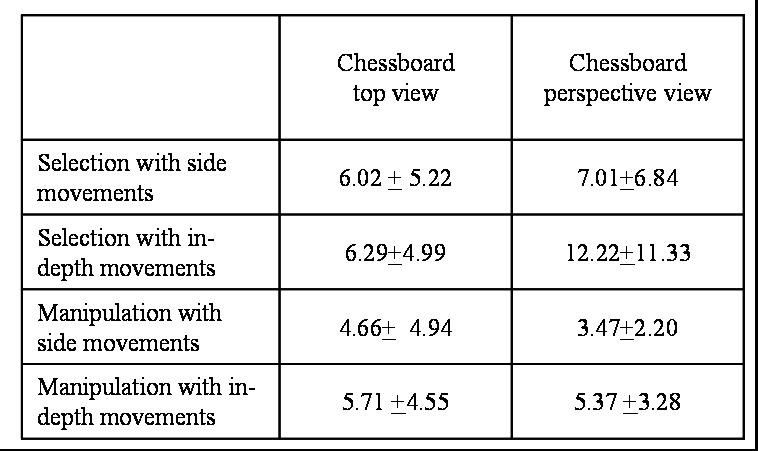
\includegraphics[width=.7\textwidth]{table.jpg}
%\end{table}

\bibliographystyle{sbc}
\bibliography{sbc-template}

\end{document}
